% select subfiles base file
\documentclass[TGAI_Laborbericht.tex]{subfiles}
\begin{document}


\begin{titlepage}

\vspace*{-3.5cm}

\begin{flushleft}
\hspace*{-1cm} 
\includegraphics[width=15.7cm]{preface/htwg-logo}
\end{flushleft}

\vspace{1cm}

\begin{center}
	\large{
		\textbf{\strLecture} \\[2cm]
	}
	\Huge{
		\textbf{\LaTeX ~Template Beispiele} \\[2cm]
	}
	\Large{
		\textbf{Martin Miller}} \\[3cm]
	\large{
		\textbf{} \\[2.3cm]
	}
	
	\large{
		\textbf{Konstanz, \strDate}
	}
\end{center}

\end{titlepage}
\thispagestyle{empty}



%
% Inhaltsverzeichnis
%
\tableofcontents

%
% Abbildungsverzeichnis
%
\phantomsection
\addcontentsline{toc}{chapter}{Abbildungsverzeichnis}
\listoffigures
\thispagestyle{lists}
\newpage

%
% Tabellenverzeichnis
%
\phantomsection
\addcontentsline{toc}{chapter}{Tabellenverzeichnis}
\listoftables
\thispagestyle{lists}
\newpage

%
% Listingverzeichnis
%
\phantomsection
\renewcommand\lstlistingname{Listing}
\renewcommand\lstlistlistingname{Listingverzeichnis}
\lstlistoflistings
\addcontentsline{toc}{chapter}{Listingverzeichnis}
\thispagestyle{lists}
\newpage

%
% Abkürzungsverzeichnis
%
\phantomsection
\addcontentsline{toc}{chapter}{Abkürzungsverzeichnis}
\twocolumn
\chapter*{Abkürzungsverzeichnis}
	\thispagestyle{lists}
	\begin{acronym}[ADC]
		\acro{ADC}{analog-to-digital converter}
\acro{AD}{Analog Digital}
\acro{DA}{Digital Analog}
\acro{TGAI}{Technische Grundlagen der angewandten Informatik}
 
	\end{acronym}
\onecolumn
\newpage


\chapter{Beispiele}
\label{chap:EINL}
\pagestyle{plain}

\section{Installation Texmaker}
Installationsanleitungen für Texmaker sind für die entsprechenden Betriebsysteme im folgenden aufgelistet:
\begin{itemize}
	\item \href{http://www.howtotex.com/howto/installing-latex-on-windows/}{http://www.howtotex.com/howto/installing-latex-on-windows/ (Windows)}
	\item \href{http://www.howtotex.com/howto/installing-latex-on-mac-os-x/}{http://www.howtotex.com/howto/installing-latex-on-mac-os-x/ (Mac OS X)}
	\item \href{https://apps.ubuntu.com/cat/applications/texmaker/}{https://apps.ubuntu.com/cat/applications/texmaker/ (Ubuntu)}
	\item \href{https://wiki.archlinux.org/index.php/LaTeX}{https://wiki.archlinux.org/index.php/LaTeX (Arch Linux)}
\end{itemize}


\section{\LaTeX ~ Hilfen}
\begin{itemize}
  \item \href{http://en.wikibooks.org/wiki/LaTeX}{http://en.wikibooks.org/wiki/LaTeX (EN)}
  \item \href{http://de.wikibooks.org/wiki/LaTeX-Kompendium}{http://de.wikibooks.org/wiki/LaTeX-Kompendium}
  \item \href{http://www.ctan.org/}{http://www.ctan.org/ (online package info)}
  \item in Eingabeaufforderung: texdoc <Packet Name>
\end{itemize}
\newpage

\section{Zitieren mit \LaTeX}
Das Quellenverzeichnis wird bei \LaTeX ~mit BibTeX generiert. BibTeX muss nach dem Compilieren der \LaTeX~ Datei (Texmaker F1) ausgeführt werden. Anschließend muss die \LaTeX~ Datei erneut compiliert werden (Texmaker F1) um das Quellenverzeichnis zu erzeugen. Die einzelnen Quellen werden in der Datei \textit{references.bib} angelegt. Es wird empfohlen hierfür das Quellenverwaltungsprogramm \href{http://jabref.sourceforge.net/}{JabRef} zu verwenden.

Im \LaTeX ~Dokument werden die Zitate wie folgt angegeben.

\raggedright Zitat (\textbackslash cite\{Franz2015\}): \linebreak
\cite{Franz2015}


\raggedright Zitat mit Seitenangabe:(\textbackslash cite[S.7]\{Franz2015a\}): \linebreak
\cite[S.7]{Franz2015a}\\
\raggedright Weitere Infos:
\begin{itemize}
	\item \href{http://en.wikibooks.org/wiki/LaTeX/Bibliography\_Management}{http://en.wikibooks.org/wiki/LaTeX/Bibliography\_Management}
	\item \href{http://jabref.sourceforge.net/}{http://jabref.sourceforge.net/}
\end{itemize}

\section{Querverweise in \LaTeX}
\raggedright Querverweise werden mit \textbackslash ref\{...\} auf ein entsprechendes Label (\textbackslash label\{...\}) angegeben (hier auf Label \textit{chap:EINL}) \linebreak
$\longrightarrow$ \ref{chap:EINL}


\section{Mathematische Formeln in \LaTeX}
Vorzugsweise sollen Formeln im Bericht wie folgt dargestellt werden.\linebreak
Formel \ref{eq:MATH_FORM}:
\begin{equation}\label{eq:MATH_FORM}
T[k]=C-A\cdot\cos\left[\frac{\pi \cdot H_{C}[k-1]}{S}\right]   \mbox{    für } k = 1,2,...,\left(2^{N}-1\right)
\end{equation}
Dabei bedeuten:
\begin{itemize}[label=]
    \item $C$: Offset Faktor
    \item $A$: Gain Faktor
    \item $S$: Sample Anzahl
\end{itemize}
Die für Formel \ref{eq:MATH_FORM} verwendeten \LaTeX ~Befehle sind in Listing \ref{lst:MATH_FORM} aufgelistet.
\begin{lstlisting}[style=LATEX, frame=single, caption=Latex Befehle für Formel \ref{eq:MATH_FORM}, captionpos=b, label=lst:MATH_FORM_LST]
\begin{equation}\label{eq:MATH_FORM}
T[k] = C - A \cdot \cos \left[ \frac{\pi \cdot H_{C}[k-1]}{S} \right]
   \mbox{    für } k = 1,2,...,\left(2^{N}-1\right)
\end{equation}
Dabei bedeuten:
\begin{itemize}[label=]
    \item $C$: Offset Faktor
    \item $A$: Gain Faktor
    \item $S$: Sample Anzahl
\end{itemize}
\end{lstlisting}

Alternativ können Formeln auch mithilfe des Mathematik Modus (\textcolor{ForestGreen}{\$...\$}) direkt eingegeben werden.\linebreak
$T[k]=C-A\cdot\cos\left[\frac{\pi \cdot H_{C}[k-1]}{S}\right]   \text{~~~~für } k \equal 1,2,...,\left(2^{N}-1\right)$
\newpage

\LaTeX ~ Befehle Listing \ref{lst:MATH_FORM_MATH_MODE}:
\begin{lstlisting}[style=LATEX, frame=single, caption=Mathematikmodus \LaTeX, captionpos=b, label=lst:MATH_FORM_MATH_MODE]
$T[k] = C - A \cdot \cos \left[ \frac{\pi \cdot H_{C}[k-1]}{S} \right]
   \mbox{    für } k = 1,2,...,\left(2^{N}-1\right)$
\end{lstlisting}
Weitere Infos:
\begin{itemize}
  \item \href{http://en.wikibooks.org/wiki/LaTeX/Mathematics}{http://en.wikibooks.org/wiki/LaTeX/Mathematics}
  \item \href{http://en.wikibooks.org/wiki/LaTeX/Advanced\_Mathematics}{http://en.wikibooks.org/wiki/LaTeX/Advanced\_Mathematics} 
  \item \href{ftp://ftp.ams.org/pub/tex/doc/amsmath/amsldoc.pdf}{ftp://ftp.ams.org/pub/tex/doc/amsmath/amsldoc.pdf}
\end{itemize}
\newpage

\section{Tabellen in \LaTeX}

\begin{lstlisting}[style=LATEX, frame=single, caption=\LaTeX ~Tabellen Prototyp, captionpos=b, label=lst:MATH_FORM]
\begin{table}[H]
\begin{tabular}{|l|l|l|l|}
...
\caption{Korrekturfaktoren zur Schätzung der 
         Messunsicherheit\cite[S.10]{Fra2014b}}
\label{tab:KORREKTURFAKTUREN}
\end{table}
\end{lstlisting}
~

\begin{table}[H]
\begin{tabular}{|l|l|l|l|}
\hline
\multicolumn{1}{|c|}{Anzahl Messungen} & \multicolumn{1}{c|}{Sicherheit P = 68,26\%} & \multicolumn{1}{c|}{Sicherheit P = 95\%} & \multicolumn{1}{c|}{Sicherheit P = 99\%} \\ \hline
2                                                              & 1,84                                                                & 12.71                                                            & 63.66                                                            \\ \hline
3                                                              & 1.32                                                                & 4.3                                                              & 9.93                                                             \\ \hline
4                                                              & 1.2                                                                 & 3.18                                                             & 5.84                                                             \\ \hline
5                                                              & 1.15                                                                & 2.78                                                             & 4.6                                                              \\ \hline
6                                                              & 1.11                                                                & 2.57                                                             & 4.03                                                             \\ \hline
7                                                              & 1.09                                                                & 2.45                                                             & 3.71                                                             \\ \hline
8                                                              & 1.08                                                                & 2.37                                                             & 3.5                                                              \\ \hline
9                                                              & 1.07                                                                & 2.31                                                             & 3.36                                                             \\ \hline
10                                                             & 1.06                                                                & 2.26                                                             & 3.25                                                             \\ \hline
15                                                             & 1.04                                                                & 2.15                                                             & 2.98                                                             \\ \hline
20                                                             & 1.03                                                                & 2.09                                                             & 2.86                                                             \\ \hline
30                                                             & 1.02                                                                & 2.05                                                             & 2.76                                                             \\ \hline
50                                                             & 1.01                                                                & 2.01                                                             & 2.68                                                             \\ \hline
80                                                             & 1.0                                                                 & 1.99                                                             & 2.64                                                             \\ \hline
100                                                            & 1.0                                                                 & 1.98                                                             & 2.63                                                             \\ \hline
unendlich                                                      & 1.0                                                                 & 1.96                                                             & 2.58                                                             \\ \hline
\end{tabular}
\caption{Korrekturfaktoren zur Schätzung der Messunsicherheit\cite[S.10]{Franz2015b}}
\label{tab:KORREKTURFAKTUREN}
\end{table}

Weitere Infos:
\begin{itemize}
  \item \href{http://en.wikibooks.org/wiki/LaTeX/Tables}{http://en.wikibooks.org/wiki/LaTeX/Tables}
  \item \href{http://www.tablesgenerator.com/latex\_tables}{http://www.tablesgenerator.com/latex\_tables}
\end{itemize}

\newpage

\section{Abbildungen in \LaTeX}

\subsection{Abbildung 1x1 Beispiel}
\begin{figure}[H]
	\centering\small
	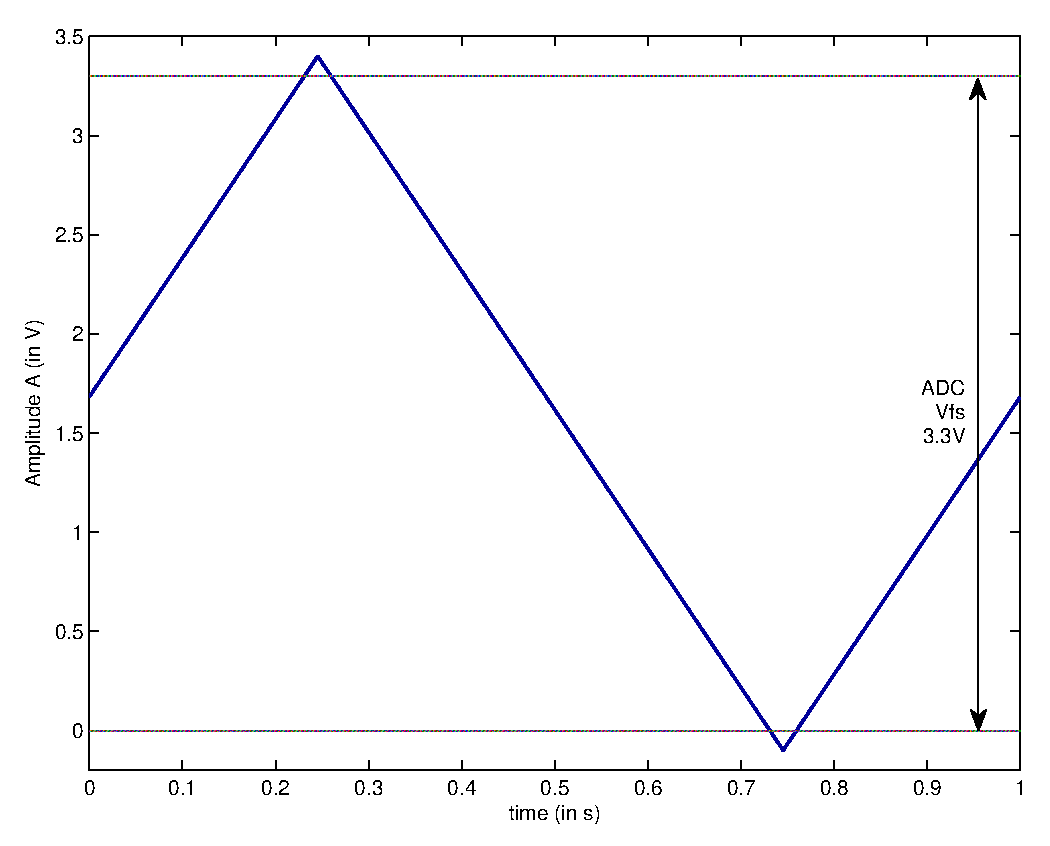
\includegraphics[width=\textwidth]{media/matlab/HISTOGRAM/ramp_fkt_samples_5000.eps}
	\caption{Eingangssignal Dreiecksfunktion}
	\label{fig:GRUNDL_RAMP_SIN_HIST_1X1}
\end{figure}
~

\begin{lstlisting}[style=LATEX, frame=single, caption=\LaTeX ~Befehle Abbildung \ref{fig:GRUNDL_RAMP_SIN_HIST_1X1}, captionpos=b, label=lst:FIG_1X1]
\begin{figure}[H]
	\centering\small
	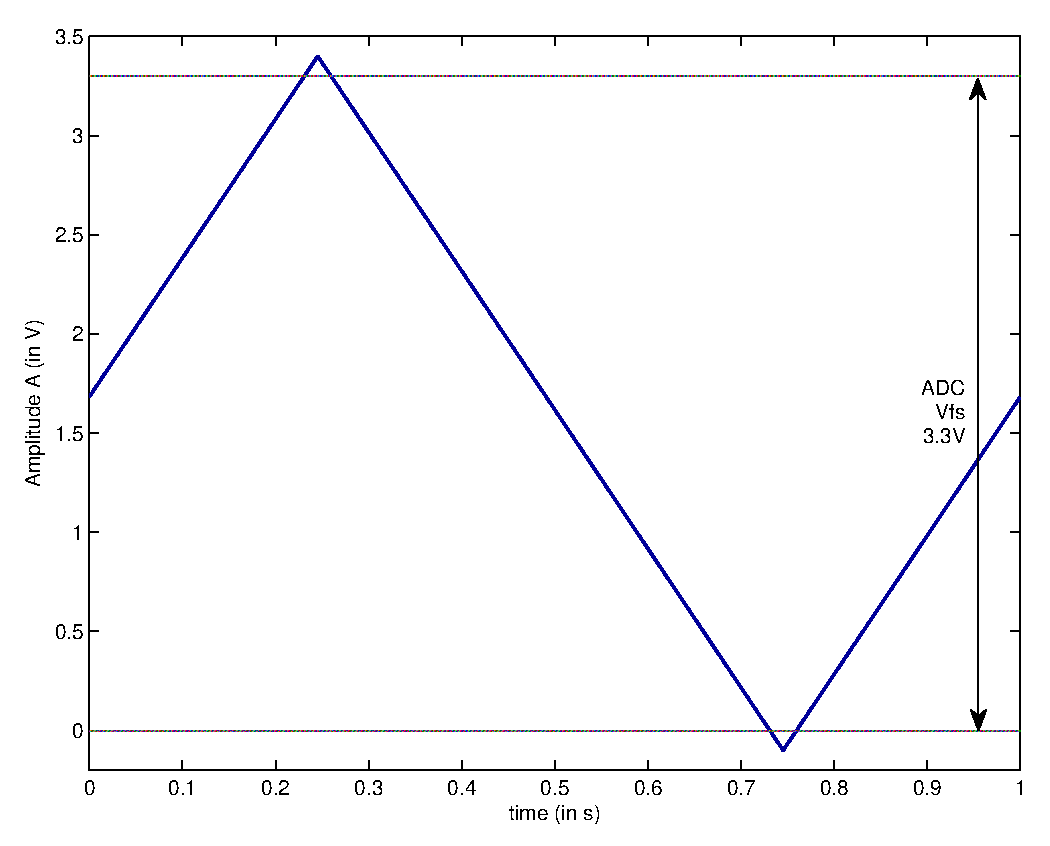
\includegraphics[width=\textwidth]{
		media/matlab/HISTOGRAM/ramp_fkt_samples_5000.eps}
	\caption{Eingangssignal Dreiecksfunktion}
	\label{fig:GRUNDL_RAMP_SIN_HIST_1X1}
\end{figure}
\end{lstlisting}
\newpage


\subsection{Abbildung 1x2 Beispiel}
\begin{figure}[H]
	\begin{subfigure}{.499\textwidth}
		\centering\small
		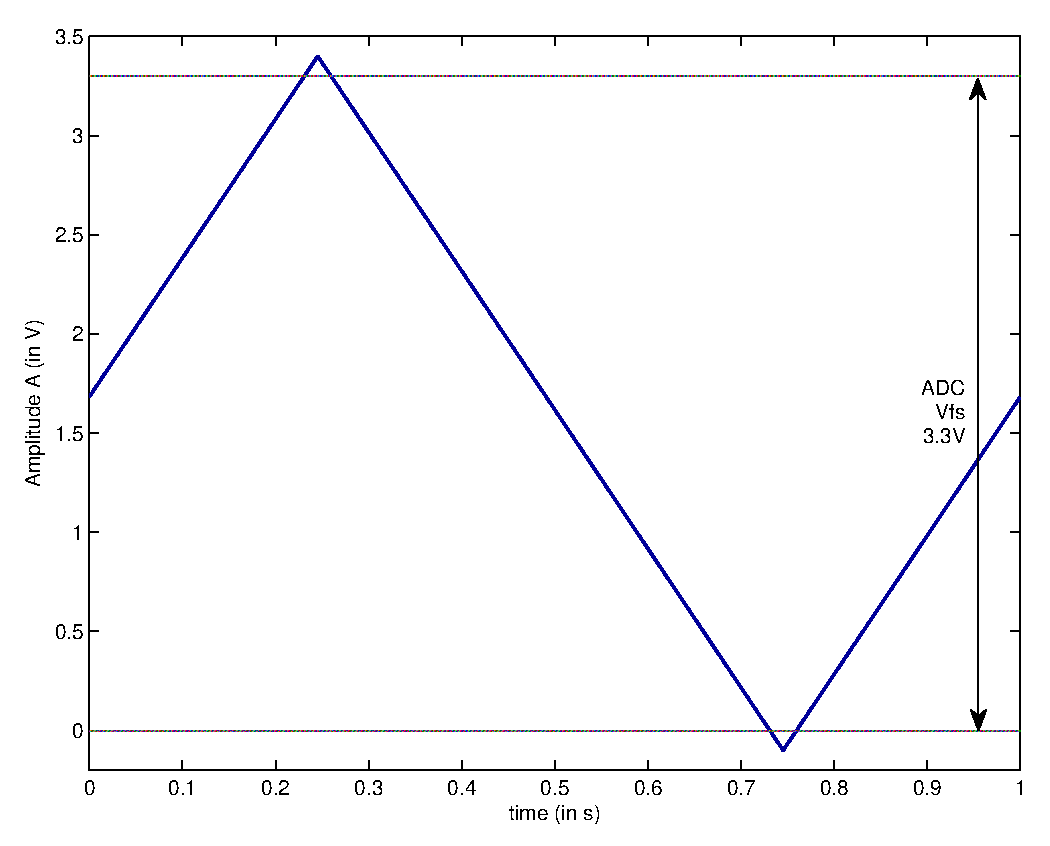
\includegraphics[width=\textwidth]{media/matlab/HISTOGRAM/ramp_fkt_samples_5000.eps}
		\caption{Eingangssignal Dreiecksfunktion}
		\label{fig:GRUNDL_RAMP_RAMP_1X2}
	\end{subfigure}
	\begin{subfigure}{.499\textwidth}
		\centering\small
		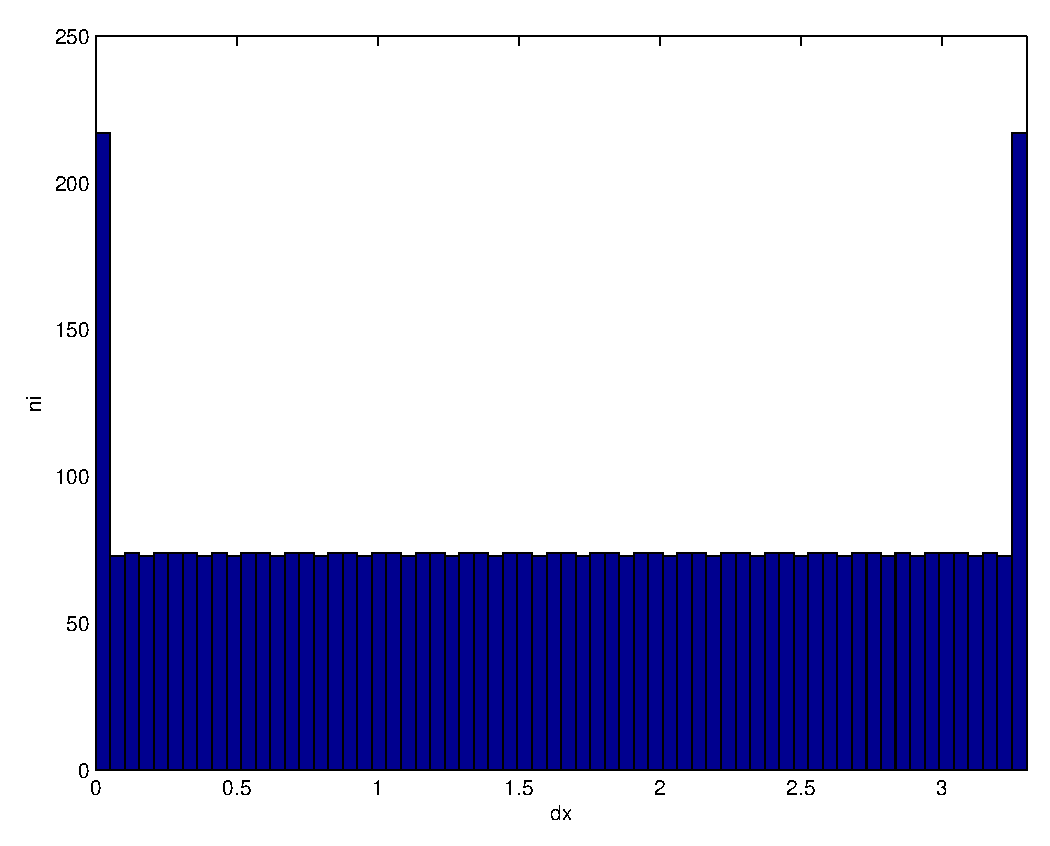
\includegraphics[width=\textwidth]{media/matlab/HISTOGRAM/ramp_hist_samples_5000.eps}
		\caption{Dreiecksfunktion Histogramm}
		\label{fig:GRUNDL_RAMP_HIST_1X2}
	\end{subfigure}
\caption{Testfunktionen mit Häufigkeitsverteilung}
\label{fig:GRUNDL_RAMP_SIN_HIST_1X2}
\end{figure}

\begin{lstlisting}[style=LATEX, frame=single, caption=\LaTeX ~Befehle Abbildung \ref{fig:GRUNDL_RAMP_SIN_HIST_1X2}, captionpos=b, label=lst:FIG_1X2]
\begin{figure}[H]
	\begin{subfigure}{.499\textwidth}
		\centering\small
		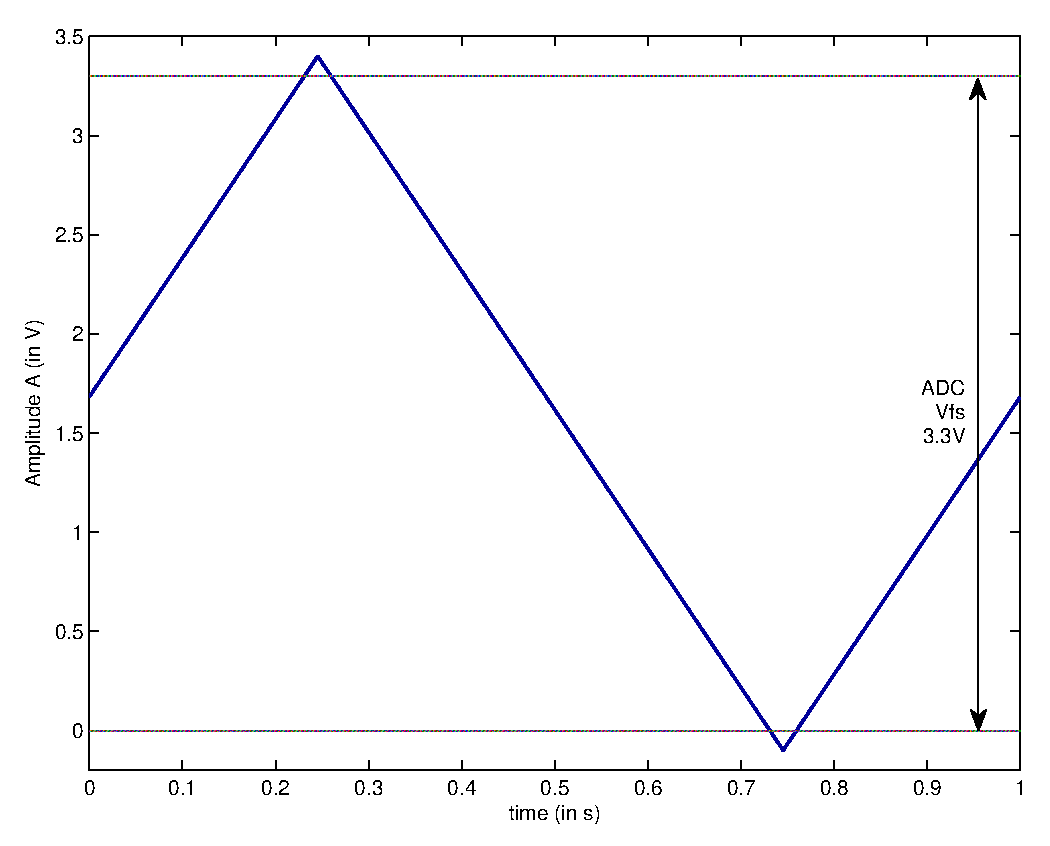
\includegraphics[width=\textwidth]{
			media/matlab/HISTOGRAM/ramp_fkt_samples_5000.eps}
		\caption{Eingangssignal Dreiecksfunktion}
		\label{fig:GRUNDL_RAMP_RAMP_1X2}
	\end{subfigure}
	\begin{subfigure}{.499\textwidth}
		\centering\small
		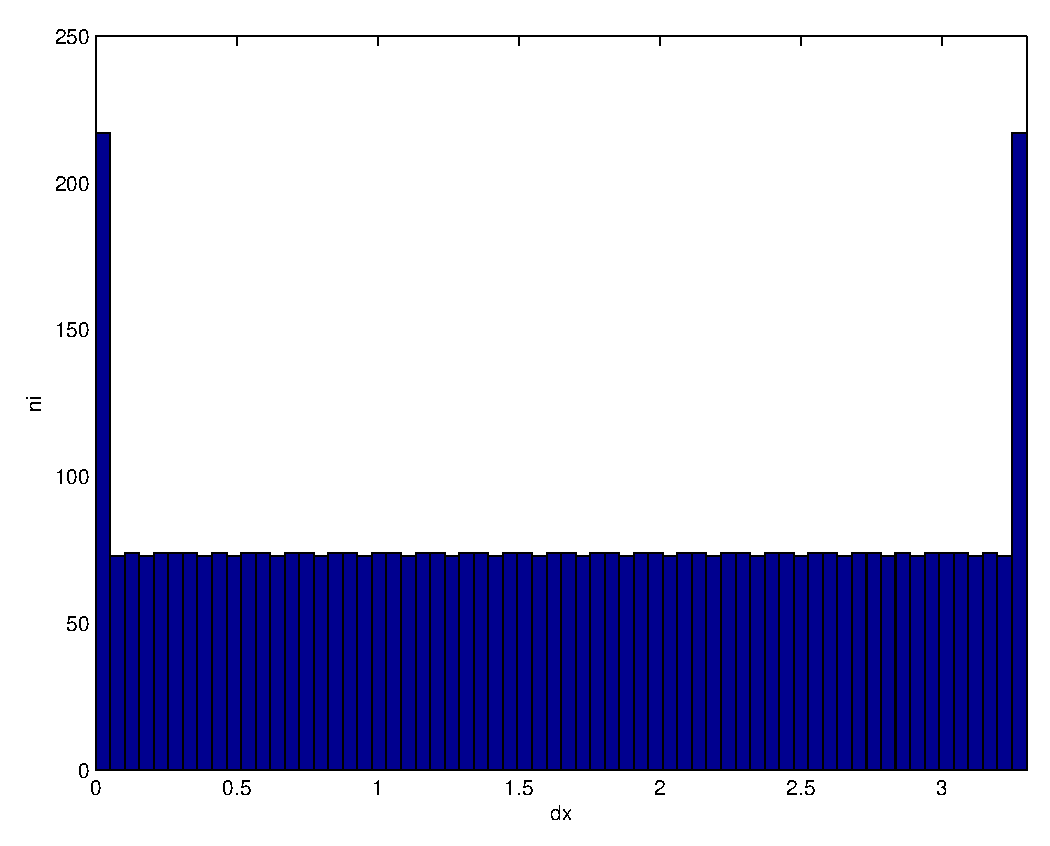
\includegraphics[width=\textwidth]{
			media/matlab/HISTOGRAM/ramp_hist_samples_5000.eps}
		\caption{Dreiecksfunktion Histogramm}
		\label{fig:GRUNDL_RAMP_HIST_1X2}
	\end{subfigure}
\caption{Testfunktionen mit Häufigkeitsverteilung}
\label{fig:GRUNDL_RAMP_SIN_HIST_1X2}
\end{figure}
\end{lstlisting}

\subsection{Abbildung 2x2 Beispiel}
\begin{figure}[H]
	\begin{subfigure}{.499\textwidth}
		\centering\small
		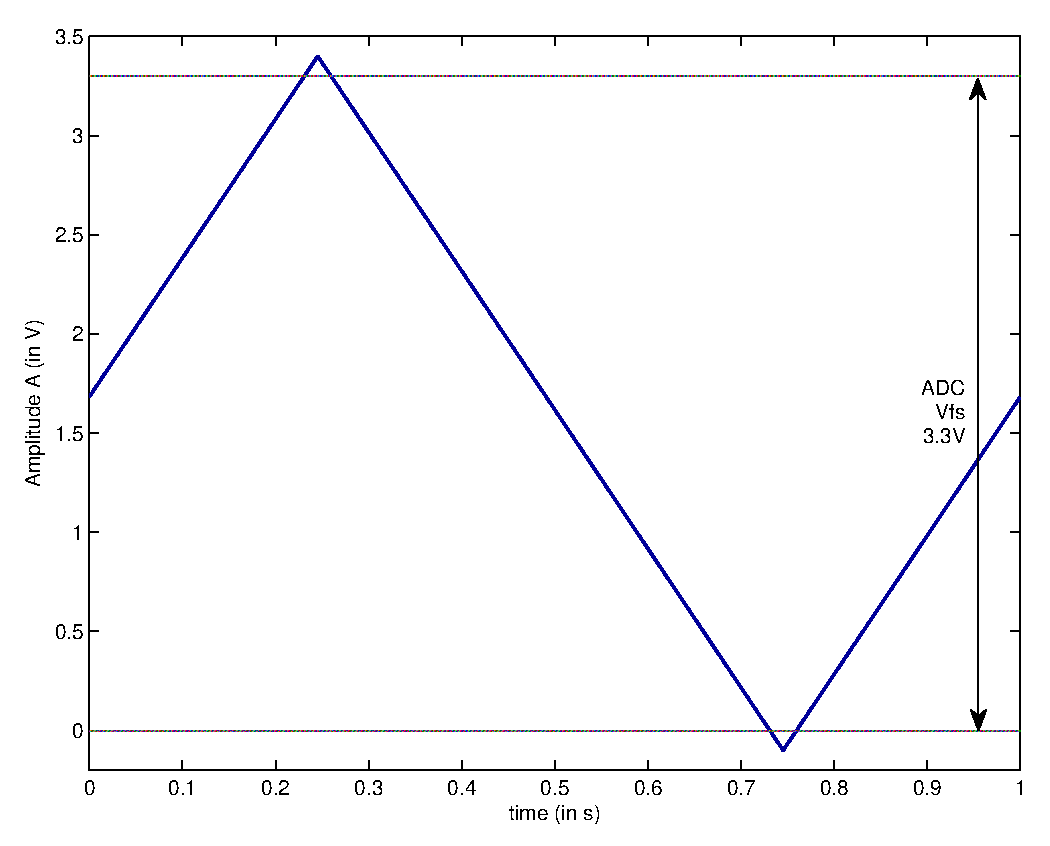
\includegraphics[width=\textwidth]{media/matlab/HISTOGRAM/ramp_fkt_samples_5000.eps}
		\caption{Eingangssignal Dreiecksfunktion}
		\label{fig:GRUNDL_RAMP_RAMP_2X2}
	\end{subfigure}
	\begin{subfigure}{.499\textwidth}
		\centering\small
		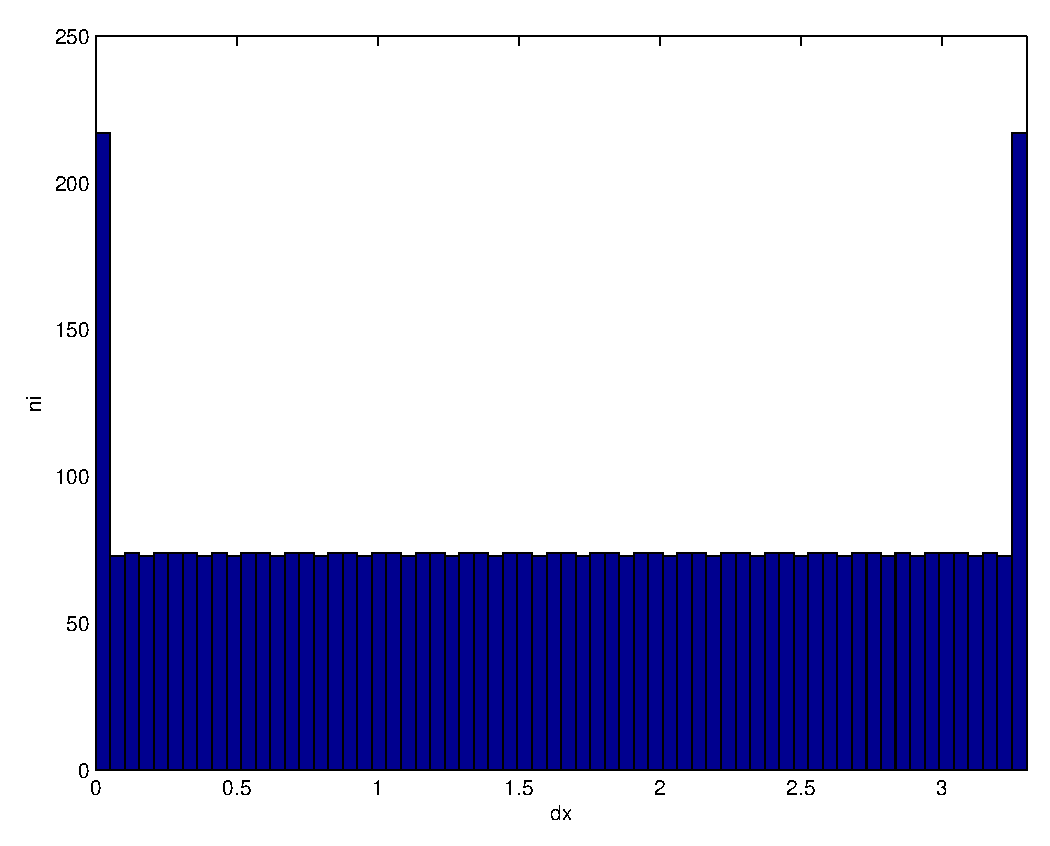
\includegraphics[width=\textwidth]{media/matlab/HISTOGRAM/ramp_hist_samples_5000.eps}
		\caption{Dreiecksfunktion Histogramm}
		\label{fig:GRUNDL_RAMP_HIST_2X2}
	\end{subfigure}
	\begin{subfigure}{.499\textwidth}
		\centering\small
		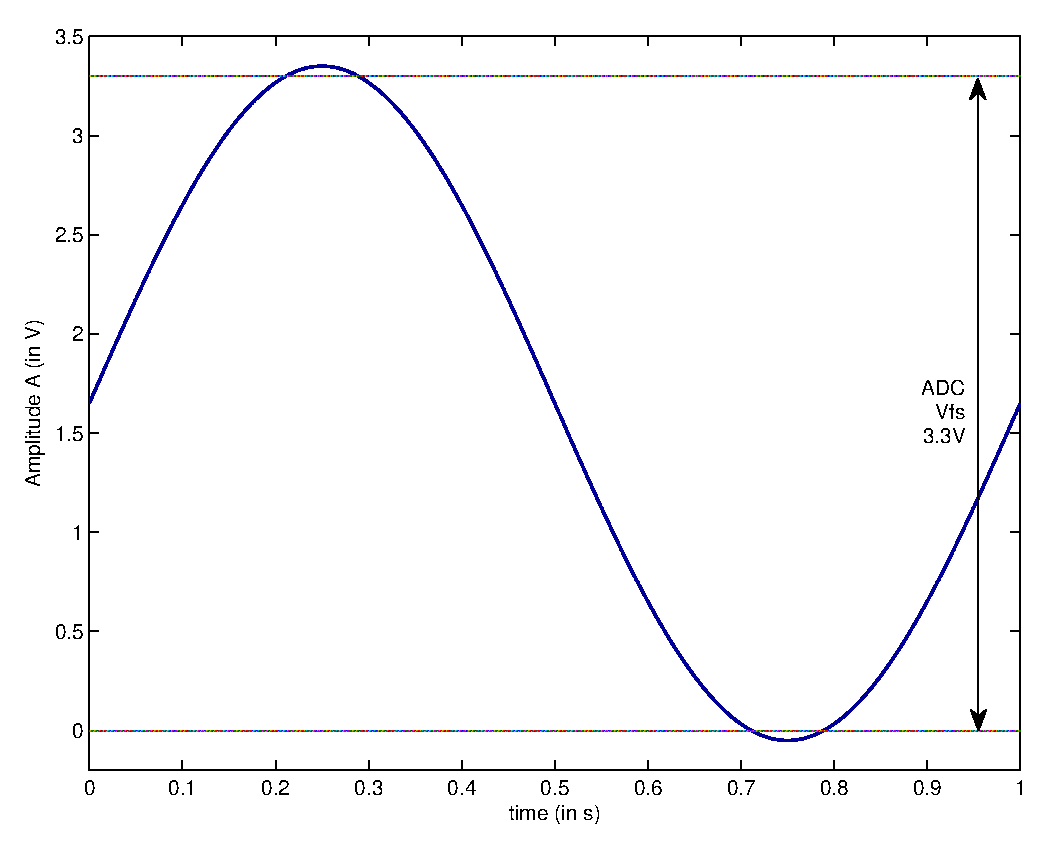
\includegraphics[width=\textwidth]{media/matlab/HISTOGRAM/sin_fkt_samples_5000.eps}
		\caption{Eingangssignal Sinus}
		\label{fig:GRUNDL_SIN_SIN_2X2}
	\end{subfigure}%
	\begin{subfigure}{.499\textwidth}
		\centering\small
		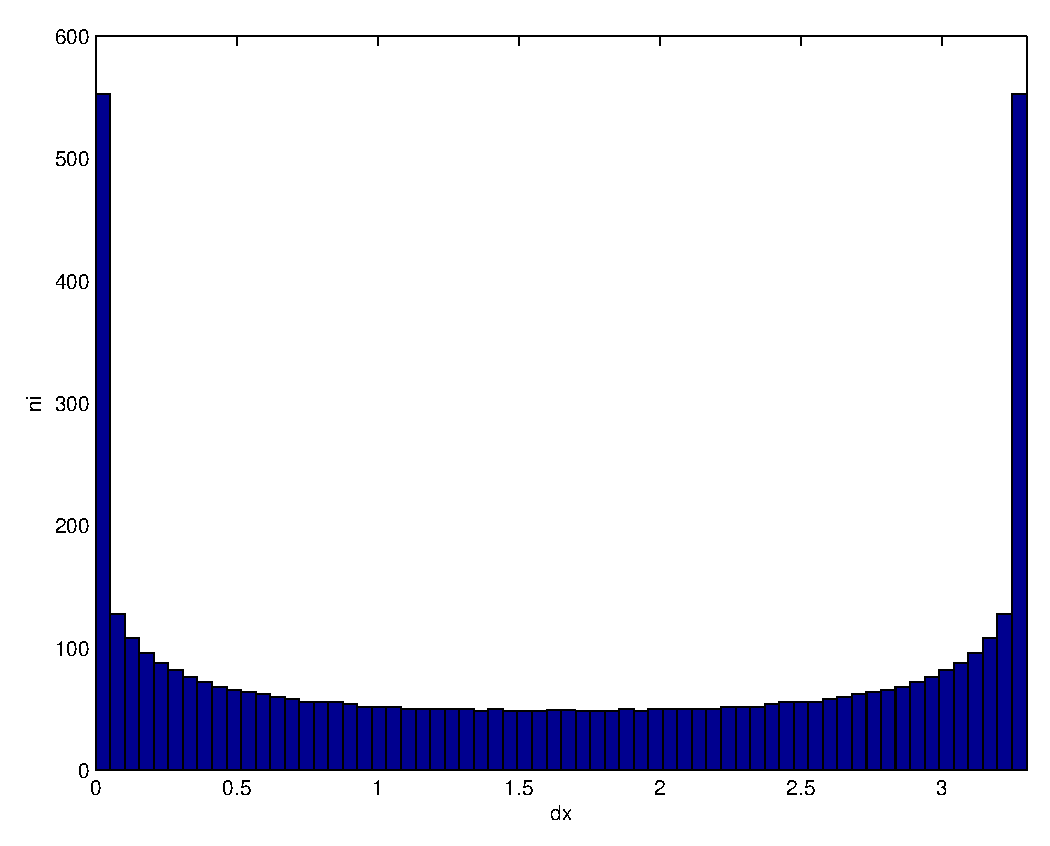
\includegraphics[width=\textwidth]{media/matlab/HISTOGRAM/sin_hist_samples_5000.eps}
		\caption{Sinus Histogramm}
		\label{fig:GRUNDL_SIN_HIST_2X2}	
	\end{subfigure}
\caption{Testfunktionen mit Häufigkeitsverteilung}
\label{fig:GRUNDL_RAMP_SIN_HIST_2X2}
\end{figure}

\subsection{Abbildung 3x3 Beispiel}
\begin{figure}[!ht]
	\begin{subfigure}{.499\textwidth}
		\centering\small
		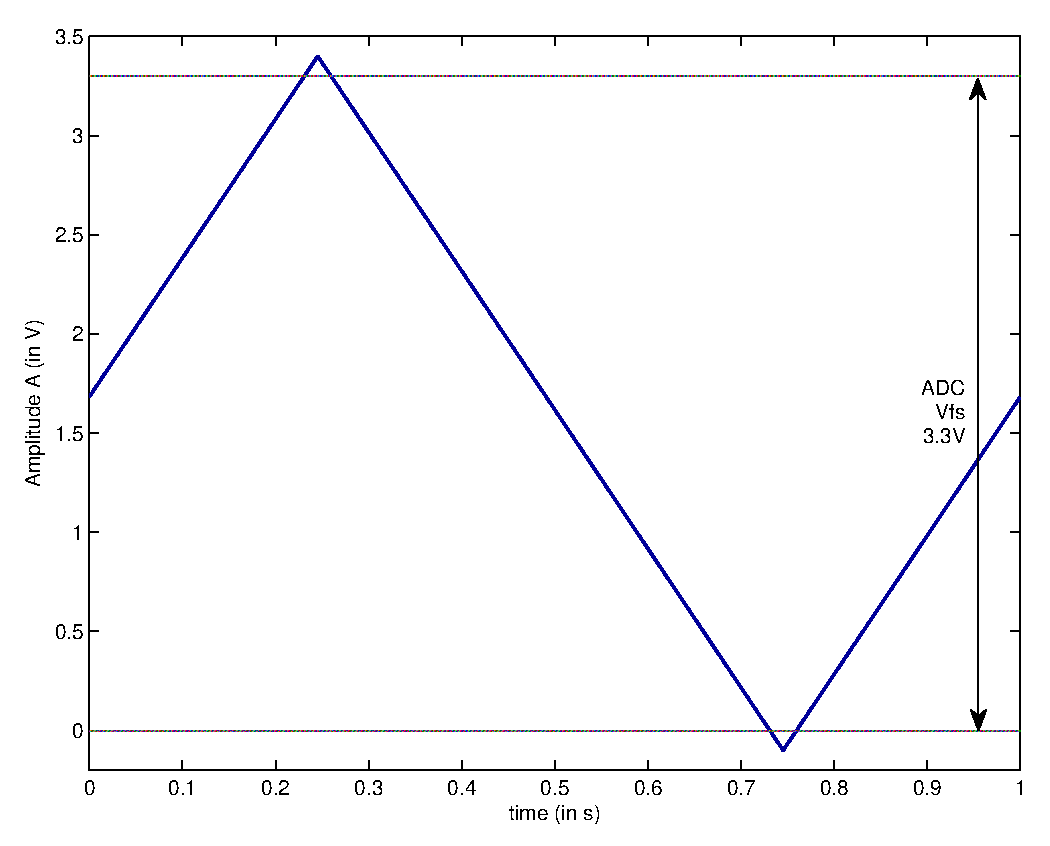
\includegraphics[width=\textwidth]{media/matlab/HISTOGRAM/ramp_fkt_samples_5000.eps}
		\caption{Eingangssignal Dreiecksfunktion}
	\end{subfigure}\label{fig:GRUNDL_RAMP_RAMP_3X3}
	\begin{subfigure}{.499\textwidth}
		\centering\small
		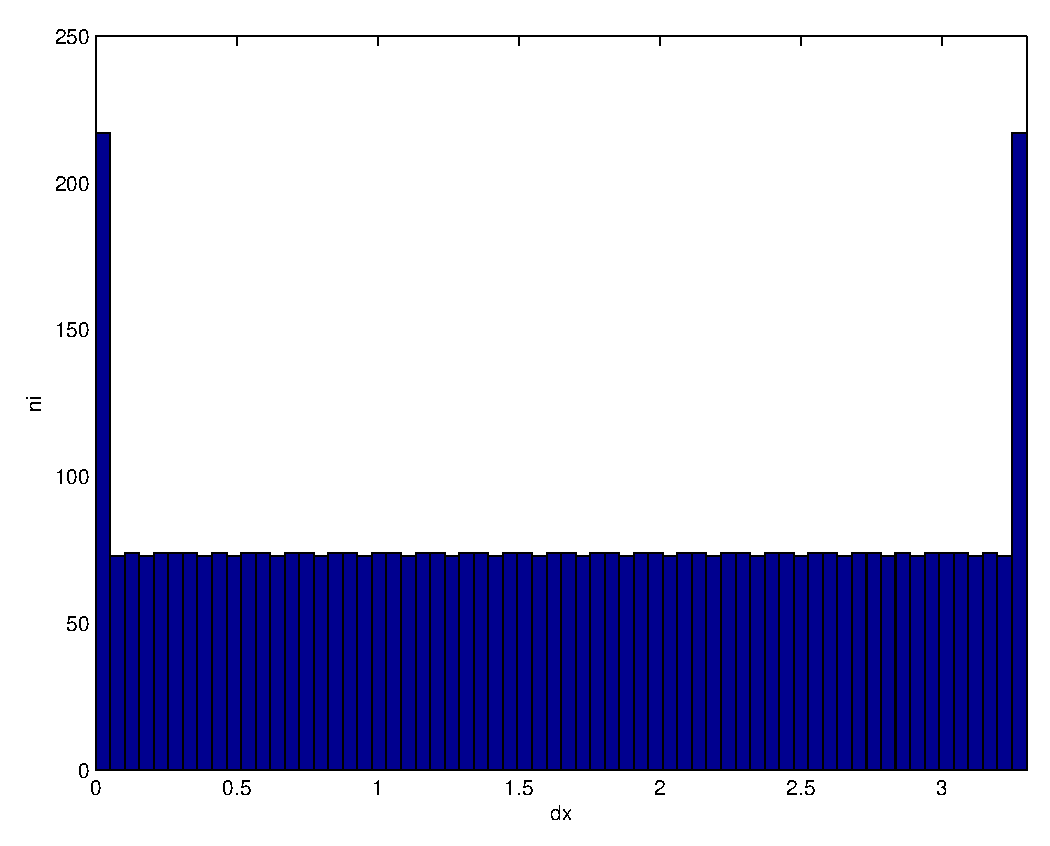
\includegraphics[width=\textwidth]{media/matlab/HISTOGRAM/ramp_hist_samples_5000.eps}
		\caption{Dreiecksfunktion Histogramm}
		\label{fig:GRUNDL_RAMP_HIST_3X3}
	\end{subfigure}
	\begin{subfigure}{.499\textwidth}
		\centering\small
		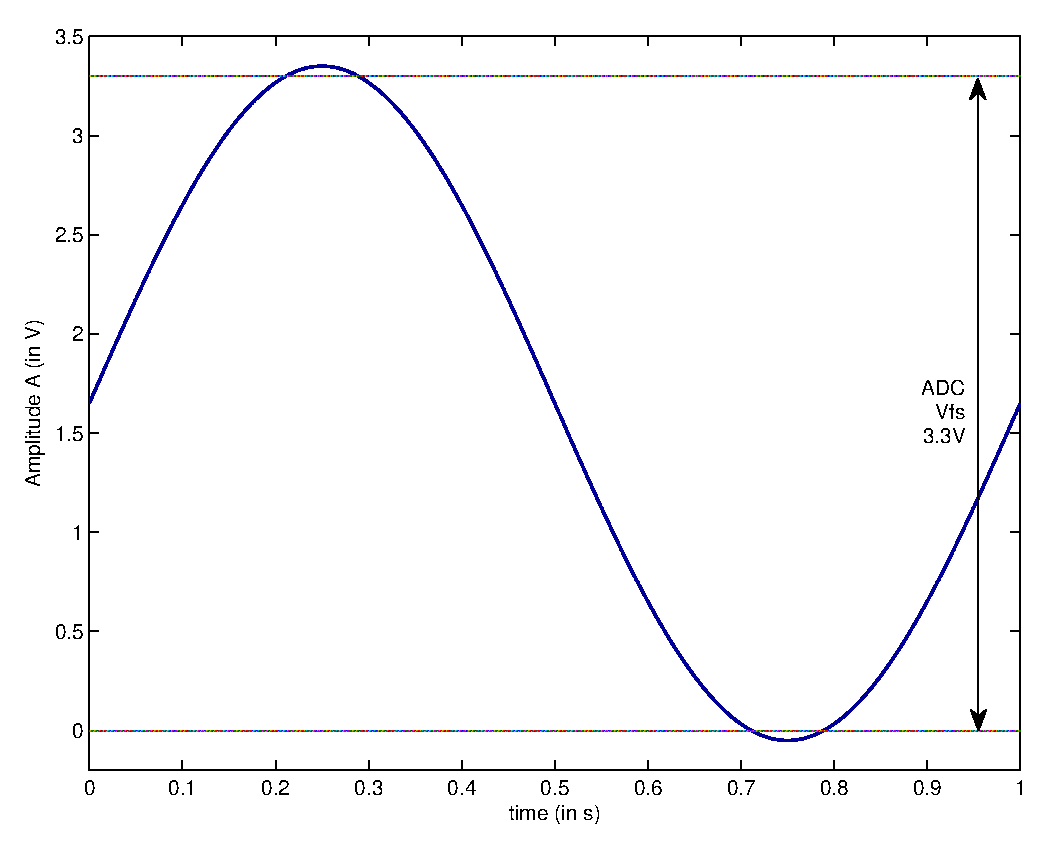
\includegraphics[width=\textwidth]{media/matlab/HISTOGRAM/sin_fkt_samples_5000.eps}
		\caption{Eingangssignal Sinus}
		\label{fig:GRUNDL_SIN_SIN_3X3}
	\end{subfigure}%
	\begin{subfigure}{.499\textwidth}
		\centering\small
		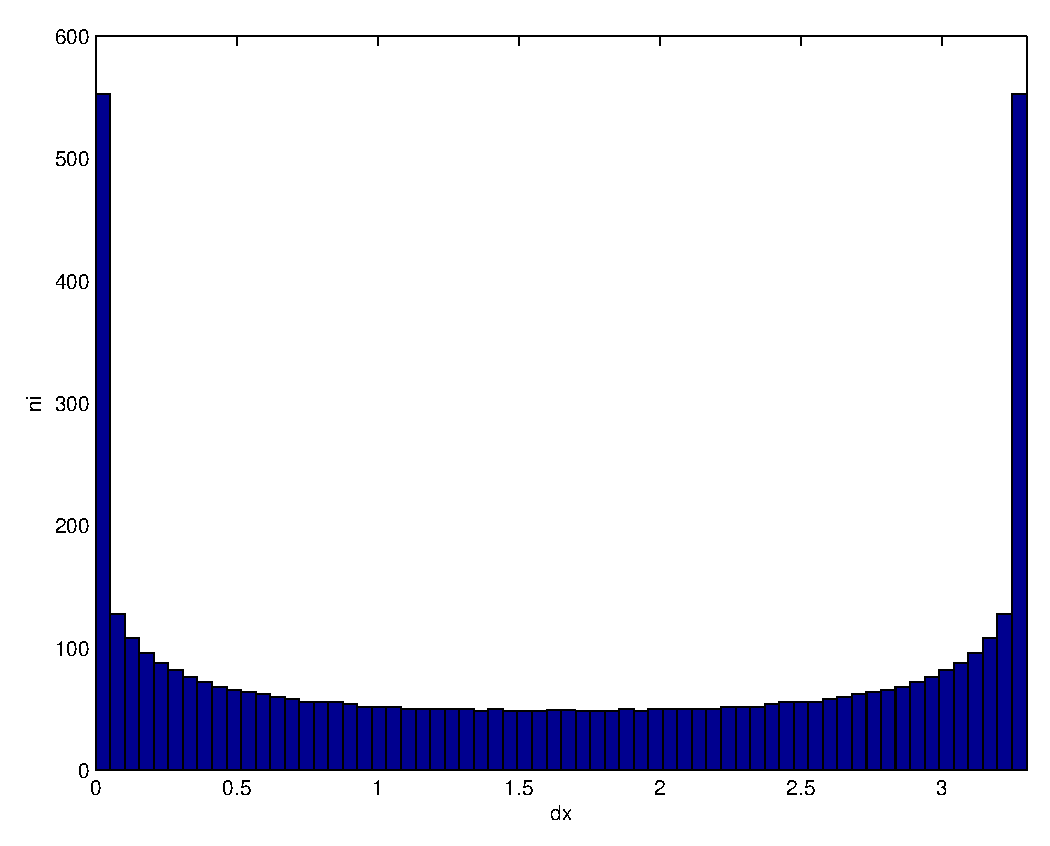
\includegraphics[width=\textwidth]{media/matlab/HISTOGRAM/sin_hist_samples_5000.eps}
		\caption{Sinus Histogramm}
		\label{fig:GRUNDL_SIN_HIST_3X3}	
	\end{subfigure}
	\begin{subfigure}{.499\textwidth}
		\centering\small
		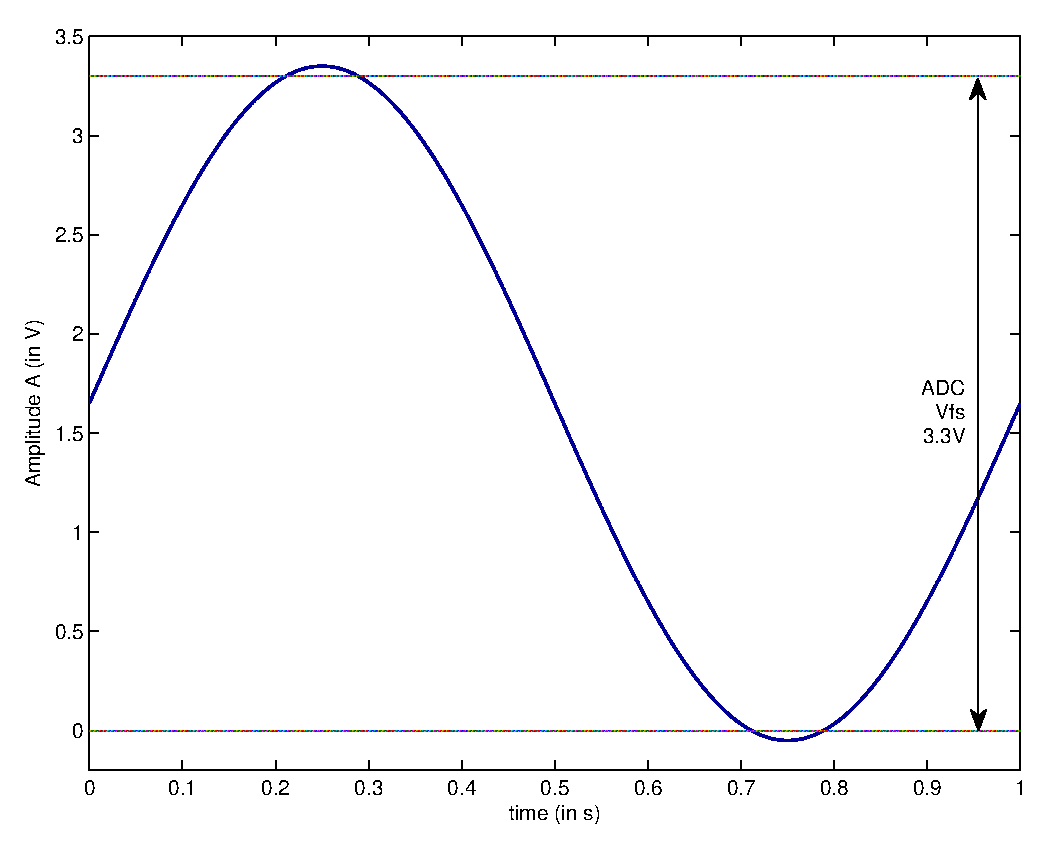
\includegraphics[width=\textwidth]{media/matlab/HISTOGRAM/sin_fkt_samples_5000.eps}
		\caption{Eingangssignal Sinus}
		\label{fig:GRUNDL_SIN_SIN_A_3X3}
	\end{subfigure}%
	\begin{subfigure}{.499\textwidth}
		\centering\small
		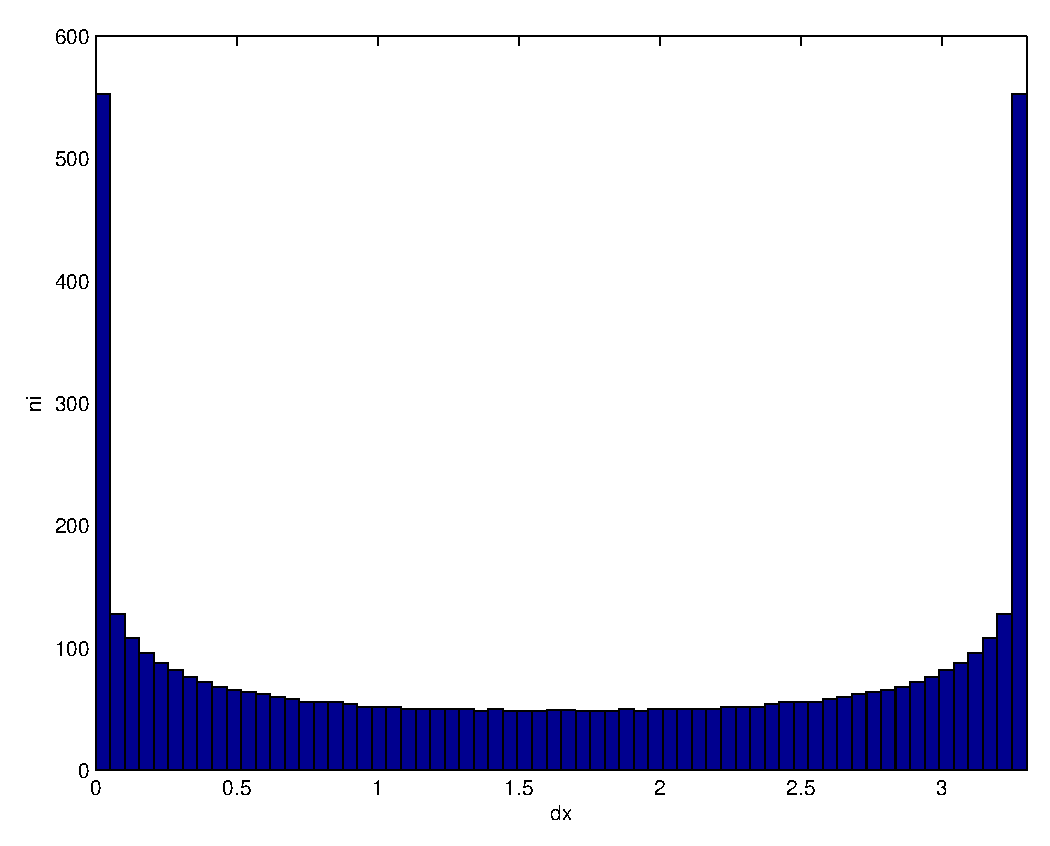
\includegraphics[width=\textwidth]{media/matlab/HISTOGRAM/sin_hist_samples_5000.eps}
		\caption{Sinus Histogramm}
		\label{fig:GRUNDL_SIN_HIST_A_3X3}
	\end{subfigure}	
\caption{3x3 Abbildung Beispiel}
\label{fig:GRUNDL_RAMP_SIN_HIST}
\end{figure}
\newpage

\section{Positionierung von Bildern und Tabellen}
Die Positionierung von Bildern und Tabellen wird in \LaTeX nach der \textit{\textbackslash begin} Anweisung in eckigen Klammern angegeben (siehe Listing \ref{lst:POS_PIC}). Hier werden die Positionierungswünsche aufgereiht. Ist ein Positionierungs-Wunsch nicht durchführbar, so wird versucht den nächsten durchzuführen.

\begin{lstlisting}[style=LATEX, frame=single, caption=Positionierung von Bildern , captionpos=b, label=lst:POS_PIC]
\begin{figure}[!htbp]
\includegraphics{filename}%
\caption{text}%
\end{figure}
\end{lstlisting}

\LaTeX unterstützt folgende Positionierungsangaben.
\begin{itemize}
	\item h -  bedeutet "here", also an der aktuellen Position
	\item H -  präzise Angabe "here", also genau an der aktuellen Position (package \textit{float})
	\item t -  bedeutet "top", also am Anfang der aktuellen Seite
	\item b -  bedeutet "bottom", also am Ende der aktuellen Seite
	\item p -  bedeutet "page",also auf einer eigenen Seite
	\item ! -  gibt an, dass intere Parameter überschrieben werden sollen
\end{itemize}

Leider ignoriert der LaTeX Compiler die Positionsangabe, wenn diese nicht durchgeführt werden kann. Dies kann in den meisten Fällen durch Angabe von mehreren alternativen Positionsangaben korrigiert werden (z.B. [!htb]). Wenn dies nichts hilft, kann weiterhin über \textit{\textbackslash newpage}  der Positionierungsbereich eingeschränkt werden. Hilft selbst dies nichts, dann kann das package float, mit
\begin{lstlisting}[style=LATEX]
\usepackage{float}
\end{lstlisting}
geladen werden. Hierdurch werden die Positionsangaben mit H immer an der aktuellen Position durchgeführt. Dies wird auch dann durchgeführt, wenn die aktuelle Seite keinen Platz mehr für das Bild hat. Das Bild wird dann auf der nächsten Seite dargestellt. Bei der Positionierung ist deshalb immer die Positionierungangabe H zu empfehlen.

Weitere Infos:
\begin{itemize}
  \item \href{http://texblog.net/latex-archive/uncategorized/prevent-floating-image-figure-table/}{http://texblog.net/latex-archive/uncategorized/prevent-floating-image-figure-table/}
\end{itemize}

\section{Source-Code Listings in \LaTeX}
Source Code Listings können in \LaTeX bequem mit dem \textit{listings} eingefügt werden. In Listing \ref{lst:SIN_PLOT} ist ein Python Listing dargestellt.
\begin{lstlisting}[style=PYTHON, frame=single, caption=Sinus Plot, captionpos=b, label=lst:SIN_PLOT]
"""
"""
X = np.linspace(-np.pi, np.pi, 256)
C,S = np.cos(X), np.sin(X)
# plot sine
fig,ax = plt.subplots()
ax.plot(X,C)
ax.plot(X,S);
ax.set_xlabel('time')
print('plot done')
\end{lstlisting}
Der Source Code kann entweder direkt in das \LaTeX Dokument kopiert werden, oder über die Source File direkt geladen werden. In Listing \ref{lst:MATLABSC_SYNTAX_HIGHL} ist die Befehlsfolge zur Darstellung des Python Codes im Latex Dokument dargestellt. 
\begin{lstlisting}[style=LATEX, frame=single, caption=Latex Source Code Syntax Highlighting Prototyp, captionpos=b, label=lst:MATLABSC_SYNTAX_HIGHL]
\begin{lstlisting}[
	style=PYTHON,
	frame=single, 
	caption=<<LISTING BEZEICHNUNG>>, 
	captionpos=b, 
	label=lst:<<LABEL>>]
<<PYTHON SOURCE CODE>>
\end{lstlisting }
\end{lstlisting}
Listing \ref{lst:MATLABSC_SYNTAX_HIGHL2} zeigt den Befehl um den Source Code von einer Datei zu laden.
\begin{lstlisting}[style=LATEX, frame=single, caption=Source Code in Latex Dokument, captionpos=b, label=lst:MATLABSC_SYNTAX_HIGHL2]
\lstinputlisting[
	style=PYTHON, 
	frame=single, 
	caption=<<LISTING BEZEICHNUNG>>, 
	captionpos=b, 
	firstline=45, 
	lastline=56, 
	firstnumber=45]{scr/sinPlot.py}
\end{lstlisting}


%
% Literaturverzeichnis
%
%
% Literaturverzeichnis
%
\phantomsection
\addcontentsline{toc}{chapter}{Literaturverzeichnis}
\bibliography{../references}
\newpage

\end{document}

